\chapter{Mercado de Trabalho}

\par Os empregos são  vetores de indicações para a atividade econômica de um país, por isso, o governo federal realiza inúmeras pesquisas sobre os empregos formais e informais. Assim, tem-se o \acrshort{caged} (Cadastro Geral de Empregados e Desempregados) que reúne inúmeras informações sobre os empregos formais, sendo, admissão, desligamento, salários, funções, cargos, etc.
\par O \acrshort{caged} é atualizado mensalmente pelo ministério do trabalho, gerando uma atualização destes dados para realização de pesquisas e prognósticos econômicos. Outro ponto, é que o \acrshort{caged} abrange tanto a unidade federativa geral, como estados e municípios, gerando uma demonstração uniforme nos dados nacionais. Nos parágrafos a seguir desta sessão, é analisado e apresentado os dados sobre os empregos do ano vigente.
\par Também usa-se os dados da \acrshort{pnadc} (Pesquisa Nacional por Amostra de Domicílios), para calcular a taxa de desemprego, ocupação, renda média dos trabalhadores. Utilizando esses conjuntos de dados será iniciado uma analise da situação do mercado de trabalho no estado do Tocantins, começando  o objetivo de se estudar o primeiro semestre de 2020 e fazendo comparativos com o primeiro semestre de 2019.

\begin{smbox}[label={labelbox},nameref={Empregos}]{Origem dos dados}
	O CAGED (Cadastro Geral de Empregados e Desempregados) tem um inicio da série em 1992 para o Brasil em geral, agora para os estados tem de inicio por volta de 1996, sempre feito pelo Ministério do Trabalho. Porém, um problema nacional é a nossa mudança de metodologias que ocorrem em decorrer desse período. O \acrshort{caged} e divulgado todos os meses, por voltado dos dias 02 até o dia 10 do mês vigente.
\end{smbox}

\par Analisando os dados do saldo de emprego até o segundo trimestre. É de se visualizar o impacto da COVID-19 nos meses que o isolamento social teve uma maior latência.

\begin{figure}[!h]
	\begin{subfigure}{\linewidth}
		\caption{Saldo de empregos ao longo de 2020}
		\subcap{Em mil.}
		\label{fig:empregos}
		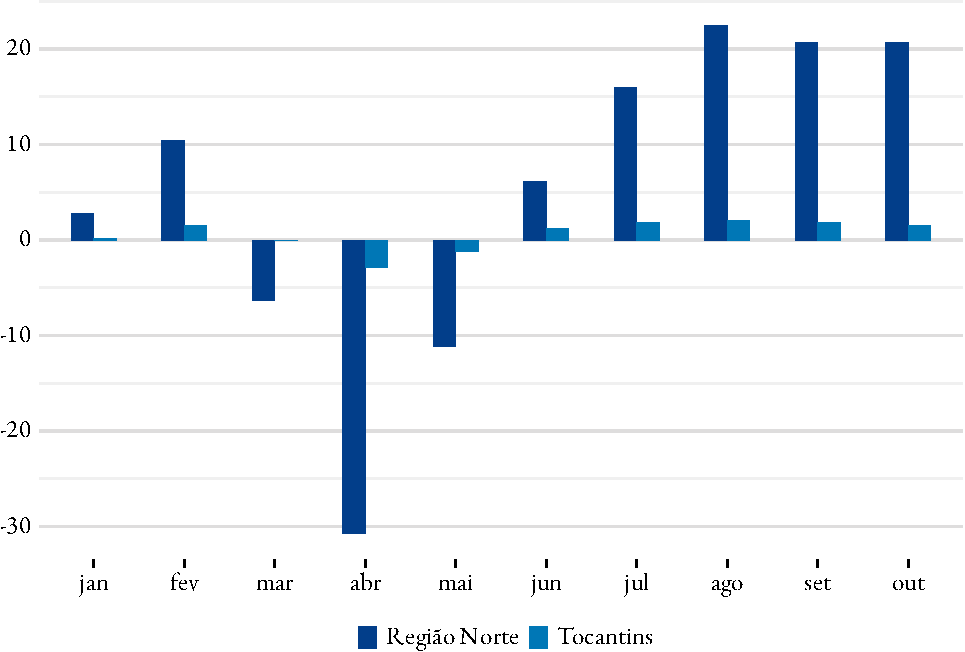
\includegraphics{fig/saldo-1.pdf}
		\source{Ministério do Trabalho}
	\end{subfigure}
	\begin{subfigure}{\linewidth}
		\caption{Saldo de empregos por setores}
		\label{fig:setores}
		\subcap{Em mil. No primeiro semestre de 2020.}
		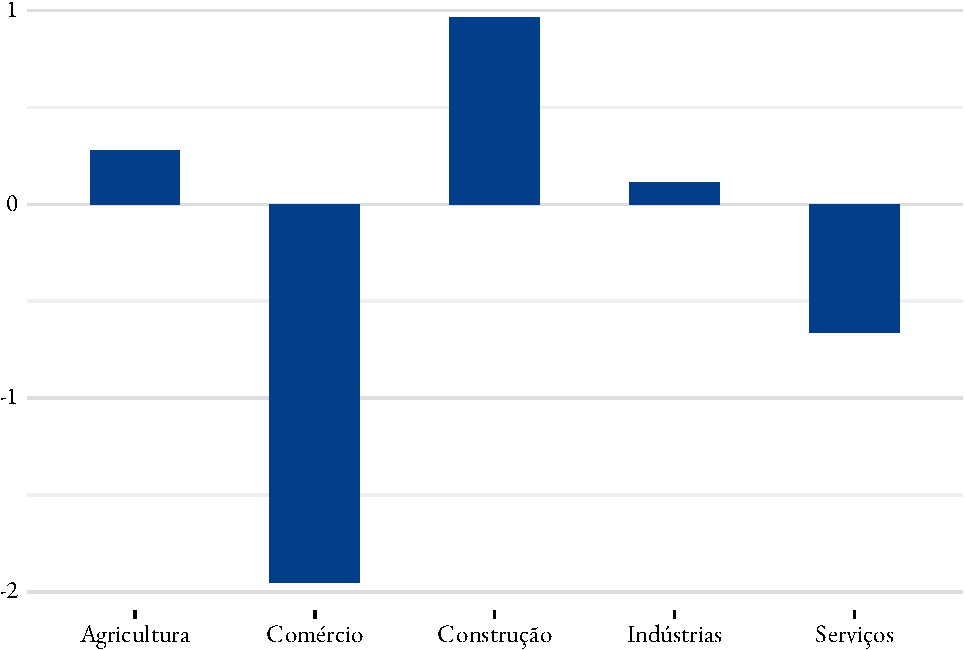
\includegraphics{fig/saldo_setor_to-1.pdf}
		\source{Ministério do Trabalho}
	\end{subfigure}
\end{figure}

\par Entendendo a situação tocantinense, observa-se que o impacto dos empregos no Tocantins foram consideráveis, gerando uma perda total de -4.127. Um impacto preocupante, porém, a partir de um afrouxamento do isolamento social ocorre uma recuperação destes empregos nos meses seguintes.

\par Já no caso da Região Norte, compreendemos um movimento bem similar ao do Tocantins, apresentado na Figura \ref{fig:empregos}. Existe uma semelhança bem especifica no período de impacto que os empregos sofreram, muito similar ao caso tocantinense. Possíveis efeitos do isolamento social para a contenção da atual pandemia.

\par Um ponto importante para entender o contexto dessas admissões e demissões é compreender os setores que mais contratam e consequentemente também demitem, na Figura \ref{fig:setores}. Por isso, é usado a \acrshort{cnae} (Classificação Nacional de Atividades Econômicas), pois realizam cortes nos setores econômicos.

\par No primeiro semestre do ano vigente, as admissões e contratações ocorreram de forma desigual nos setores econômicos, alguns lidaram de forma melhor com os efeitos do Covid-19 e outros não conseguiram recuperar os postos de trabalhos perdidos. Demonstrando a importância do setor na economia tocantinense, apresentando um saldo negativo de -1.984 vagas no período semestral, o comércio foi o setor mais impactado pela crise econômica. Conforme, relatado nas primeiras sessões, a economia tocantinense tem um perfil voltado para os serviços, comércio e a agricultura, uma visualização destas variações é apresentado na Figura \ref{fig:setores}. Se o comércio e os serviços apresentaram resultados negativos, outros setores conseguiram se destacar no meio da pandemia. Agricultura, construção civil e a indústria obtiveram resultados positivos, sendo o segundo com um saldo de 996 contratações.


\par Com o saldo apresentado na Figura \ref{fig:setores}, é necessário entender a formação dos admitidos e demitidos, como a faixa etária e o gênero. A Tabela \ref{tab:idadesEgeneros} apresenta esses dados e as suas variações. No primeiro semestre do ano, indivíduos com faixa etária entre 14 a 34 anos, tiveram mais postos de trabalhos disponíveis, com um valor bruto de 12.933 contratações. Com uma predominância masculina nestas vagas, com um valor total de 11.043. E por fim, os admitidos tinham uma formação maior no ensino médio completo com um total de 20.158 vagas.

\par Já nos desligamentos, a faixa etária que sofre mais com as demissões são trabalhadores da faixa etária de 14 até 34 anos, similar aos admitidos. O valor total das demissões nessa faixa etária é de 11.375, número inferior ao de admitidos, gerando um saldo positivo de 1.558 vagas. Já no componente do gênero, os homens apresentaram as maiores demissões, com 11.043 e um saldo positivo de 174 postos de trabalho. As mulheres, entretanto conseguiram manter seus empregos e tiveram um saldo maior, com 507 vagas. Já no quesito formação acadêmica, é bem similar aos admitidos, na qual pessoas com ensino médio completo foram os maiores contratados, neste caso, as demissões foram superiores, ocorreu uma perda de postos de trabalhos de 21.228 vagas e um saldo negativo de -1.070 para quem tem ensino médio completo. 


\begin{table}

	\caption{\label{tab:idadesEgeneros}Perfil dos Admitidos e Demitidos no CAGED}
	\subcap{Dados acumulados do primeiro semestre de 2020.}
	\begin{tabu} to \linewidth {>{\raggedright}X>{\raggedleft}X>{\raggedleft}X>{\raggedleft}X}
		\toprule
		& Admitidos & Demitidos & Saldo\\
		\midrule
		\addlinespace[0.3em]
		\multicolumn{4}{l}{Idade}\\
		\hspace{1em}14-34 & 12.933 & 11.375 & 1.558\\
		\hspace{1em}35-65 & 5.270 & 5.677 & -407\\
		\hspace{1em}65+ & 21 & 59 & -38\\
		\addlinespace[0.3em]
		\multicolumn{4}{l}{Sexo}\\
		\hspace{1em}Homem & 11.043 & 10.869 & 174\\
		\hspace{1em}Mulher & 6.243 & 5.736 & 507\\
		\addlinespace[0.3em]
		\multicolumn{4}{l}{Escolaridade} \\
		\hspace{1em}A & 108 & 109 & -1\\
		\hspace{1em}F.C & 1.727 & 1.816 & -89\\
		\hspace{1em}M.I.C & 1.997 & 2.321 & -324\\
		\hspace{1em}M.C & 20.158 & 21.228 & -1.070\\
		\hspace{1em}S.C & 2.332 & 2.106 & 226\\
		\hspace{1em}P.G  & 168 & 130 & 38\\
		\bottomrule
	\end{tabu}
	\source{Ministério do Trabalho}
	\notes{A: Analfabetos, F.C: Fundamental completo, M.I.C: Médio incompleto, M.C: Médio completo, S.C: Superior completo, P.G: Pós-graduação}
\end{table}


\par As mulheres conseguiram manter os seus empregos, mesmo havendo menos contrações do que os homens, um ponto interessante desse primeiro semestre é de como as mulheres conseguiram manter os seus empregos formais do que os homens. Outro ponto observado é a variação de empregos pela escolaridade, na tabela \ref{tab:idadesEgeneros} foi apresentado as maiores variações, entretanto, os dados por escolaridade tem outras separações além do que foi apresentado na tabela, são esses, até o quinto ano incompleta, o quinto ano completo, do sexto ao nono ano, superior incompleto, mestrado e doutorado. Essas classificações tiveram uma menor variação comparado ao que foi apresentado na tabela \ref{tab:idadesEgeneros}.


\begin{smbox}[label={labelbox},nameref={Desigualdade por gênero}]{Desigualdade por gênero no mercado de trabalho}
	Já é um tópico bem usual que o mercado de trabalho formal é um quanto desigual para as mulheres, existe uma vasta literatura sobre desigualdades salarias, vagas de empregos, oportunidades, etc. Alguns estudos buscam interpretar o efeito que uma equidade no mercado de trabalho possa gerar na economia como tudo, estudos que provocam essa afirmativa tendem a afirmar que o mercado de trabalho brasileiro é desigual em oportunidades e por consequência na renda. Na literatura ainda é possível fazer cortes e analisar que essa desigualdade envolvem também localidades, etnia, grau de instrução e um outro fator que está em evidência é o capital humano herdado pelos pais e como isso gera oportunidades melhores aos filhos desses pais com instrução elevada. 
	\footnote{Abram, L. (2006). Desigualdades de gênero e raça no mercado de trabalho brasileiro.}
	
\end{smbox}



\par Outro ponto apresentado é o saldo de empregos por etnia, na Figura \ref{fig:sel2020} é observado o movimento de empregos por diferentes etnias, como também é visto situações em que os indivíduos não preferem declarar a sua etnia. Pessoas que se declararam pardas, tiveram maiores perdas de postos de trabalho, com um valor de 654 vagas, seguidas por brancos, pretos e não informados. Já o único saldo positivo é de indivíduos preferiram não informar a sua etnia, e com um valor correspondente de 545 vagas de trabalho. Concluindo a apresentação dos dados oriundos do \acrshort{caged}, um adendo importante para se entender é que as profissões onde ocorrem as maiores contratações são auxiliares de escritório, operadores de caixa, faxineiros, vendedores de comércios varejistas, serventes de obras, motoristas de caminhão e assistentes administrativos.


\begin{figure}[!h]
\begin{subfigure}{\linewidth}
	\caption{Saldo de empregos por etnia}
	\subcap{Em mil. No primeiro semestre de 2020}
	\label{fig:sel2020}
	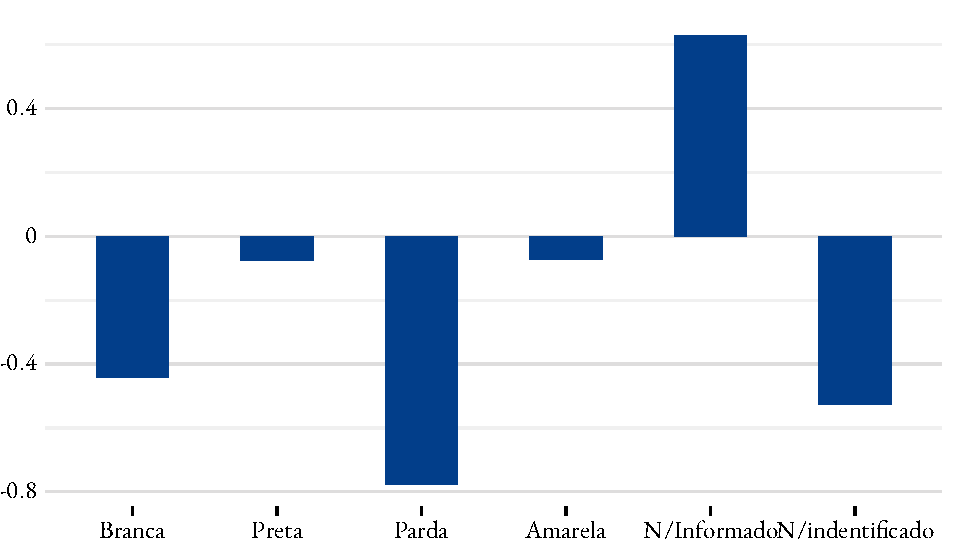
\includegraphics{fig/Saldo por etnia.pdf}
	\source{Ministério do Trabalho}
\end{subfigure}
\end{figure}




\subsection{Ocupação}

\par A taxa de desemprego é fornecida pela \acrshort{pnadc}. É divulgada pelo \acrshort{ibge} de forma trimestral e para todos os estados da federação, ela calcula a população ocupada pela desocupação, assim, estimulando a taxa de desemprego. No curso do boletim, será exposto a atual taxa de desemprego tocantinense.

\begin{figure}[!h]
	\begin{subfigure}{\linewidth}
		\caption{Taxa de desemprego no Tocantins}
		\subcap{Variaçao trimestral}
		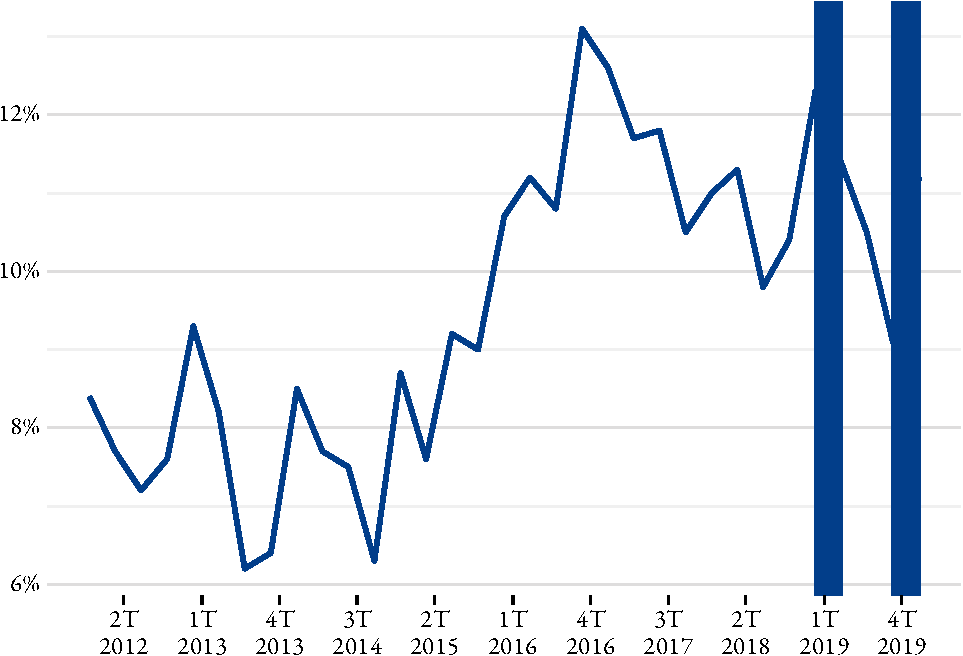
\includegraphics{fig/tx_desemprego_to-1.pdf}
		\source{\acrshort{ibge}}
		\label{fig:desemprego}
	\end{subfigure}
	\begin{subfigure}{\linewidth}
		\caption{População ocupada no Tocantins}
		\subcap{Variaçao trimestral}
		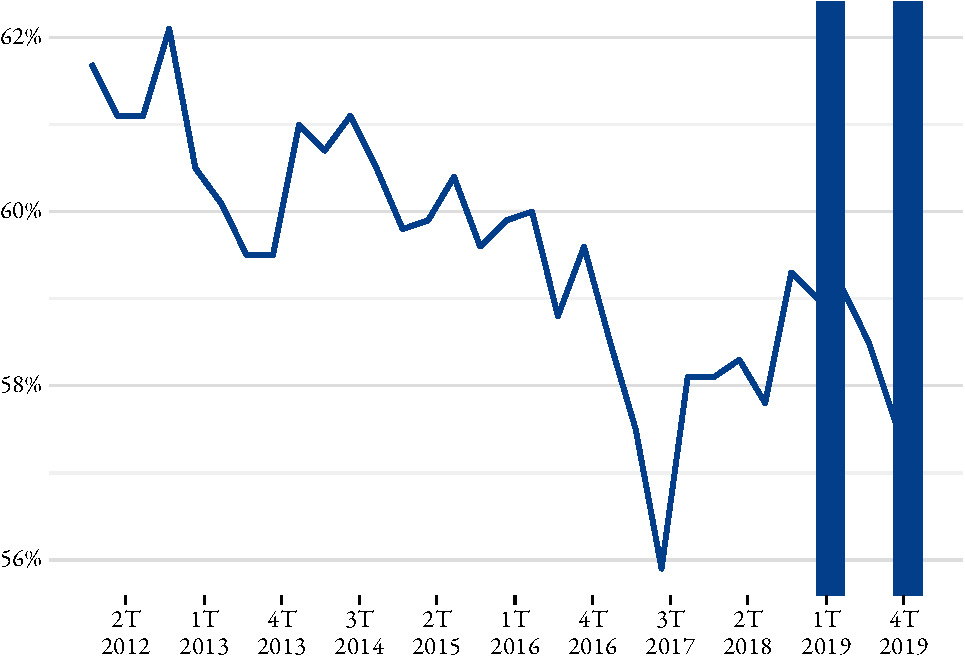
\includegraphics{fig/pop_ocupada-1.pdf}
		\source{\acrshort{ibge}}
		\label{fig:ocupada}
	\end{subfigure}
	\begin{subfigure}{\linewidth}
		\caption{Pedidos de seguro desemprego}
		\subcap{Em mil}
		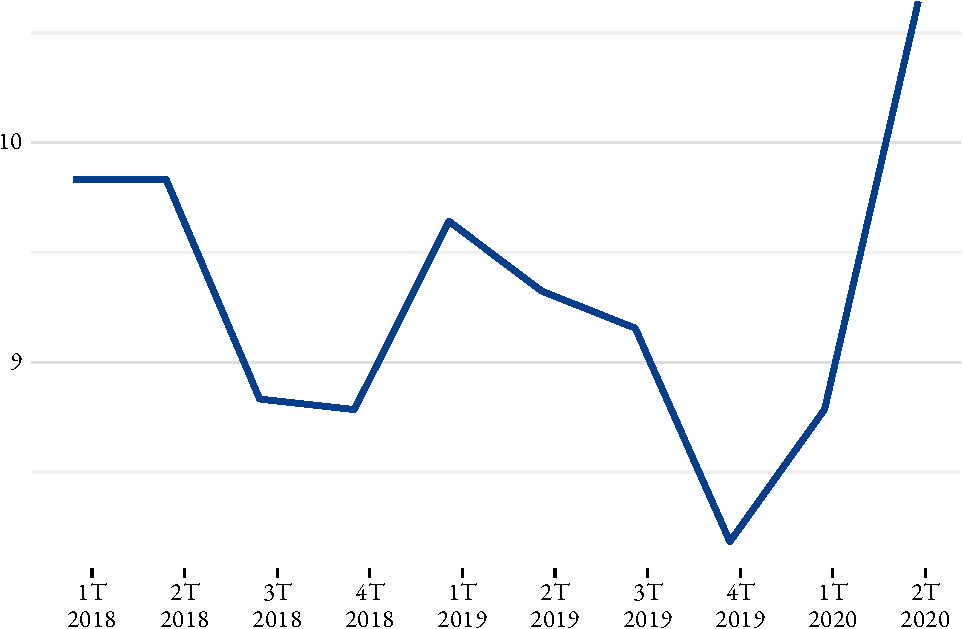
\includegraphics{fig/pedido_segudo_desem-1.pdf}
		\source{\acrshort{ibge}}
		\label{fig:seguro}
	\end{subfigure}
\end{figure}

\par A taxa de desemprego no Tocantins estava num movimento de queda a partir do primeiro trimestre de 2019, conforme a figura \ref{fig:desemprego}, porém, a partir do quarto trimestre de 2019 até o primeiro trimestre de 2020 ocorre um movimento de elevação da taxa de desemprego.



\par Outro termômetro claro para o setor de empregos são os pedidos seguro-desemprego, são apresentados na figura \ref{fig:seguro}, uma politica macroeconômico para gerar uma segurança branda para o trabalhador recém demitido. Num contexto mais claro, significa que se ocorre uma elevação dos pedidos seguro desemprego, significa que o mercado de trabalho não está em um bom funcionamento. O inverso é bem intuitivo, se a poucos pedidos é uma reação a um bom momento econômico.

\par Fazendo uma comparação com a taxa de desemprego, é apresentado a noção de que a taxa se eleva e gera um aumento nos pedidos de seguro desemprego, uma demonstração clara de como a taxa é crucial para a avaliação macroeconômica. Realiza-se uma regressão para definir o quão importante é a taxa de desemprego em relação ao seguro desemprego, para o seguinte caso:

\begin{figure}[h]
	\caption{Relação taxa de desemprego x pedidos seguro desemprego}
	\subcap{No primeiro semestre de 2020.}
	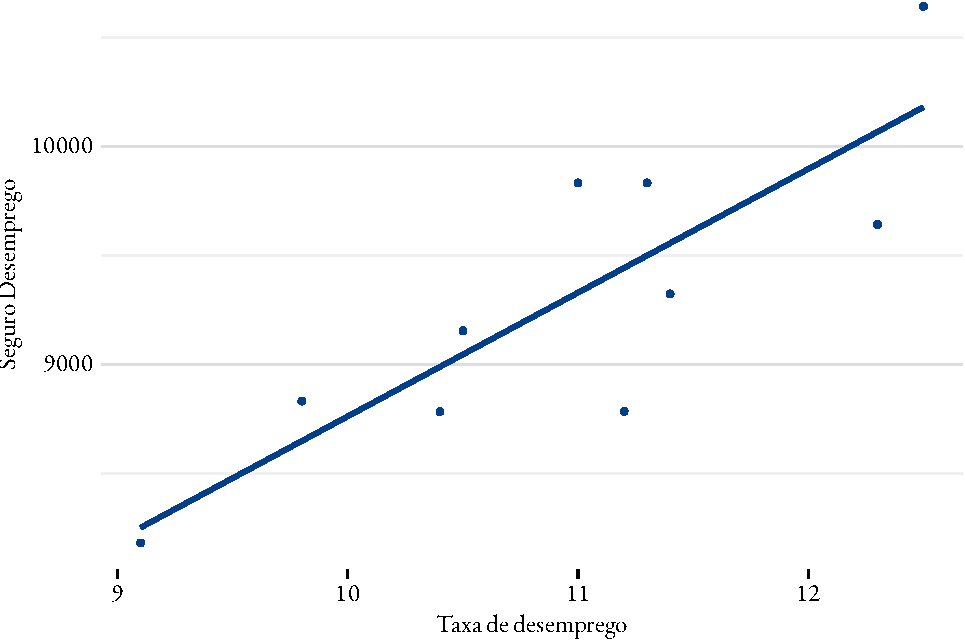
\includegraphics[width=\linewidth]{fig/reg_emprego-2.pdf}
	\source{Ministério do Trabalho}
\end{figure}
\begin{smbox}[label={labelbox},nameref={Desigualdade por gênero}]{Metódos econométricos}
	Usando uma técnica para provar a correlação da taxa de seguro desemprego e pedidos de seguro desemprego. Essa técnica é a regressão linear simples, quando existe apenas uma variável resposta e uma variável explicativa, por isso chama-se de regressão linear simples. A formula é determinada por $y = \alpha + \beta x$ e $\beta = \overline{y} - \overline{\alpha x}$.
	\\
	Por fim, utilizando um processo econométrico vemos que a relação é forte, para se ter a ideia o \textbf{R} que é referente ao processo de correlação nos aponta um número de 0,70 (quanto mais próximo de 1 for, mais forte é a relação) e o \textbf{R}$^{2}$ é de 0,66. Ou seja, essa correlação é muito forte.
\end{smbox}



\par Outro ponto crucial é a população economicamente ativa ocupada, é uma demonstração da população economicamente ativa que está trabalhando.



\par  A taxa de ocupação tocantinense, conforme a figura \ref{fig:ocupada} é bem estável pelos dados, sempre na faixa de 60\%, o que demonstra uma certa estabilidade dessa população. Comparando a taxa do primeiro trimestre de 2019, foi de 59\% e no prímeiro trimestre de 2020 foi de 57,5\%. Uma queda percentual da população ocupada.



\par O rendimento médio do Tocantins é derivado dos rendimentos dos trabalhadores, nele, é possível de se pensar na renda que esses agentes produzem. É fruto do trabalho da nossa população ocupada, sejam trabalhos principais ou habituais.

\begin{figure}[!h]
	\begin{subfigure}{\linewidth}
		\caption{Rendimento médio real}
		\subcap{Em mil R\$}
		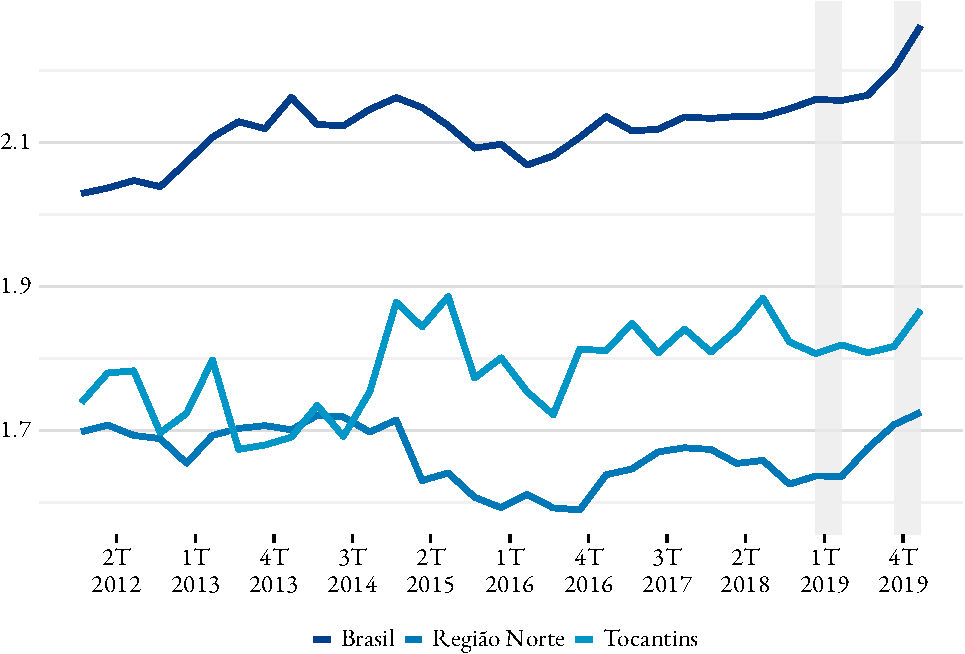
\includegraphics{fig/rend_medio-1.pdf}
		\source{\acrshort{ibge}}
	\end{subfigure}
\end{figure}


\par A renda dos trabalhadores tocantinenses está na faixa dos R\$ 1.700,00 e R\$ 1.800,00 por alguns anos, no primeiro período de 2019, a renda foi de R\$ 1.807,00 e no primeiro trimestre de 2020, foi de R\$ 1.867. Ou seja, a partir do primeiro trimestre de 2019, houve um ganho de renda muito considerável. É claro que o rendimento médio comparado com outros estados brasileiros é bem baixa, iremos comparar com a renda da região norte e do Brasil em geral.


\par A região Norte tem uma renda média menor que a do estado do Tocantins, por exemplo, no primeiro trimestre de 2019, a renda nortenha foi de R\$ 1.637,12 e no primeiro trimestre de 2020 o resultado de R\$ 1.725,25. Houve um aumento de renda desses trabalhadores, mas, abaixo do Tocantins.



\par No caso da renda média nacional, acontece um "gap" maior, a renda nacional no primeiro trimestre de 2019 foi de R\$ 2.159,51 e no primeiro trimestre de 2020, foi de R\$ 2.261,29. A região Norte e o estado do Tocantins estão com um nível de renda menor que o Brasil no geral, mas, a renda média nacional é puxada por regiões que o desenvolvimento é maior e por consequência, uma maior produtividade. Os eixos nacionais (Sul e Sudeste) tem os seus níveis de renda maiores.
